%% ############################################################################
%% Unterkapitel
%% ############################################################################
\section{ Web-Programmierschnittstelle (Web-API)}
Für die neue Webseite und für andere Anwender ist eine API (application programming interface) erstellt worden. Um eine API zu entwickeln muss zuerst verstanden werden was eine API ist. Deswegen werden zu beginn folgende Fragen gestellt und beantwortet.
\begin{itemize}
\item Was ist eine API?
\item Wie wird eine API entwickelt?
\item Was ist state of the Art?
\end{itemize}

Anschliessend wird in diesem Kapitel aufgezeigt, wie die API entwickelt wurde und wo diese zum Einsatz kommt.

\subsection{Was ist eine API?}
Eine API überbrückt die Schnittstellen zwischen verschiedenen Software teilen und strukturiert die dabei anfallende Datenübergabe dazwischen. Sie ermöglicht es, Software zu modularisieren und die Kommunikation zu vereinfachen. Konkret heisst dies, dass die einzelnen Programmteile  voneinander abgekapselt werden und kommunizieren nur über die Festgelegte API. Der Vorteil hierbei ist es, dass die API veröffentlicht werden kann. Somit kann auch anderen die Möglichkeit gegeben werden die angebotenen Dienste mittels der API zu erhalten. Zusätzlich können so auch die einzelnen modularisierte Softwareteile unabhängig voneinander weiterentwickelt werden. Nicht zuletzt ist auch das Testen ein wichtiger Punkt. Da alle Programmteile nur über die API miteinander kommunizieren sollten, muss die Software auch nur in der Zusammenarbeit mit der API getestet werden.

\subsection{Was ist state of the Art?}
Heutzutage werden viele API nach dem RESTful Standard entwickelt wird. Da taucht die Frage auf was ist RESTful? Ein kleiner Exkurs. RESt steht für State Transfer und ist im Gegensatz zu Protokollen eine Philosophie, welche die Möglichkeiten von HTTPS ausnutzt. REST benötigt hierfür die von HTTPS bekannten Verben (GET, POST, PUT, PATCH, DELETE) \cite{LornaJaneMitchell2013oreilly}. Im Vordergrund bei REST steht die Zustandslosigkeit, dass heisst Server sowie Client haben keinen Zustand zwischen den Anfragen. Eine Verbindung bleibt jedoch bis zum Ende der Anwendung oder Nutzzeit bestehen. Ein Beispiel für diese Zustandslosigkeit ist in Abb. \ref{img:Sequenzdiagramm_API} zu sehen.\\

\begin{figure}[h!]
	\centering
	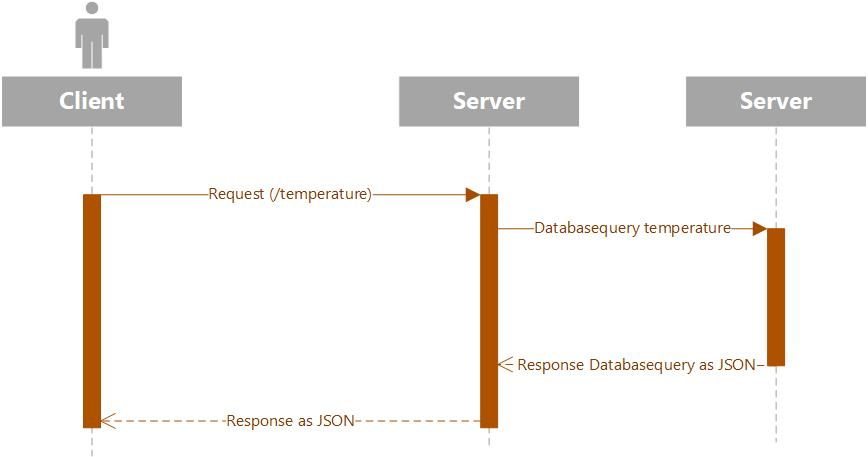
\includegraphics[width=1\linewidth]{img/Sequenzdiagramm_API}
	\caption{Beispiel einer API GET-Abfrage}
	\label{img:Sequenzdiagramm_API}
\end{figure}


\subsection{Wie wird eine API entwickelt?}
Zu Beginn der Entwicklung muss klar sein, für was die API benötigt wird. Ist dies klar, kann gesagt werden welche Anforderungen die API erfüllen muss. Als nächstes muss ein URL Schema her. Dies wird benötigt, um nach dem REST Standard zu arbeiten. Die URL sollte folgendermassen aussehen: \\ https://api.wetter-arbon.ch/Versionsnummer/Endpunkt\\
Die Versionsnummer wird zur Weiterentwicklung benötigt. Wird beispielsweise eine neue Version der API veröffentlicht, kann es sein, dass nicht alle Nutzer der API auf die neue Version umgestiegen sind. Somit kann es geschehen, dass die vorhandenen Installationen zerstört werden. Neben der URL ist es wichtig, dass die Kommunikation in einem bestimmten Datenformat erfolgt. Hier besteht die Möglichkeit zu wählen zwischen JSON, XML oder CSV zu wählen. Es können auch andere Formate genutzt werden. Wichtig ist jedoch, dass der Server sowie der Client wissen welches Format genutzt wird. Nebst der Entwicklung für die Server-Client Kommunikation ist auch bei der API eine Zugangskontrolle bzw. eine Grundbasis in der Sicherheit notwendig. Neben der Möglichkeit HTTPS zu verwenden, ist es zusätzlich möglich den Client über einen sogenannten Authorization Token zu authentifizieren.\\


\subsection{API Konzept}
Nachdem die Fragen zur API beantwortet sind, kann die API für die Wetterstation Arbon Konzipiert und umgesetzt werden. Für die API gibt es jedoch eine wichtige Bedingung. Sie muss in php geschrieben werden, da Hostpoint kein Javascript auf der Serverseite erlaubt.

Zu Beginn des API Konzept sollten die Anforderungen daran erstellt werden. Die API soll mindestens folgende Datenpunkte enthalten:
\begin{itemize}
\item Wind / Windrichtung
\item Niederschlag
\item Temperatur / Gefühlte Temperatur
\item Luftfeuchtigkeit
\item Wassertemperatur (1m Unter der Wasseroberfläche)
\item Wassertemperatur (Oberfläche)
\item Wasserpegel
\item Wellenhöhe
\item Radiation /daily sunduration
\item Webcam
\item Sturmwarnung
\end{itemize}
Die Datenabfrage über die API soll, wie es State of the Art entwickelt wird, RESTful sein und mittels HTTP geschehen. Mit der API werden nur GET-Anfragen erlaubt sein, da bspw. keine POST-Befehle oder sonstige Befehle ausgeführt werden müssen. Somit ist ein sogenannter Token für die Authentifizierung nicht notwendig. Das Datenformat der API soll JSON sein. JSON ist ein simples Datenformat, welches nicht viel Speicherplatz benötigt und somit auch einfach Transferiert werden kann. Nebst der Lesbarkeit für Menschen, kann es auch von Maschinen gelesen werden. Javascript beispielsweise handhabt JSON nativ. Nebst dem das Javascript JSON versteht, ist auch die Handhabung bei PHP simpel, wie bei PHP Web Services \cite{LornaJaneMitchell2013oreilly} erwähnt wird. 

\paragraph{JSON Struktur}

Um die API zu entwickeln, wurden die Anforderungen in einen sogenannten JSON-tree (siehe Anhang Listing \ref{lst:JsonTree}) umgeformt. Hieraus wird auch die URL entstehen zur Abfrage der Daten. Der Aufruf wird Grundsätzlich über api.wetter-arbon.ch gemacht. Um einzelne Werte abzufragen muss tiefer in die Verzeichnisse gegangen werden.


\subsection{Funktionsweise der API}

In diesem Kapitel wird die Funktionsweise nach der Umsetzung des API-Konzepts erklärt. Die ganze API ist Modular aufgebaut, dass diese für weitere Anwendungen oder Messwerte ausgebaut werden kann. Dies beginnt schon beim Verzeichnis (Abb. \ref{img:APIVerzeichnis}) .


\begin{figure}[h!]
	\centering
	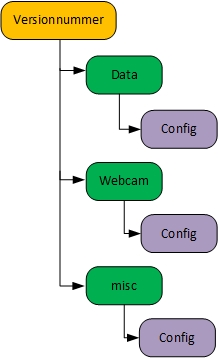
\includegraphics[width=0.3\linewidth]{img/APIVerzeichnis.jpg}
	\caption{Aufbau des API Verzeichnis}
	\label{img:APIVerzeichnis}
\end{figure}

Das Verzeichnis V1 beinhaltet drei Unterverzeichnisse, data, misc und webcam. Im Verzeichnis Data wird das JSON der Sensoren aufgebaut, im Verzeichnis Webcam wird das JSON für die Webcam erstellt. Dies ist auch das einzige Verzeichnis welches nicht auf die Datenbank zugreift. Im Verzeichnis misc werden verschiedene Arten von Daten, welche von dritten abgegriffen werden verarbeitet. Nebst dem Verzeichnis, welches modular aufgebaut ist, enthalten auch die Dateien eine gewisse Struktur. Jedes Verzeichnis config enthält die folgenden vier Dateien. 
\begin{itemize}
\item path.php
\item createJson.php
\item databaseQuery.php
\item database.php
\end{itemize}

Erfolgt eine GET-Abfrage eines Clients läuft dies gemäss Abb. \ref{img:APIFiles}  ab. Nach der GET-Abfrage wird das Routing anhand des URL Pfades im path.php vorgenommen. Im Case wird der entsprechende Funktionsaufruf mit den Parametern an das CreateJSON übergeben. Hier entsteht zum Schluss auch das JSON. Die Funktion CreateJson...() stellt das JSON nach der Datenbankabfrage read...() in der Datei databaseQuery.php her. Das JSON wird aus dem dynamischen Array, enthält die Messwerte, sowie dem statischen Array, enthält die Einheit und Beschreibung, zusammengesetzt und zurück gegeben. 

\begin{figure}[h!]
  \fbox{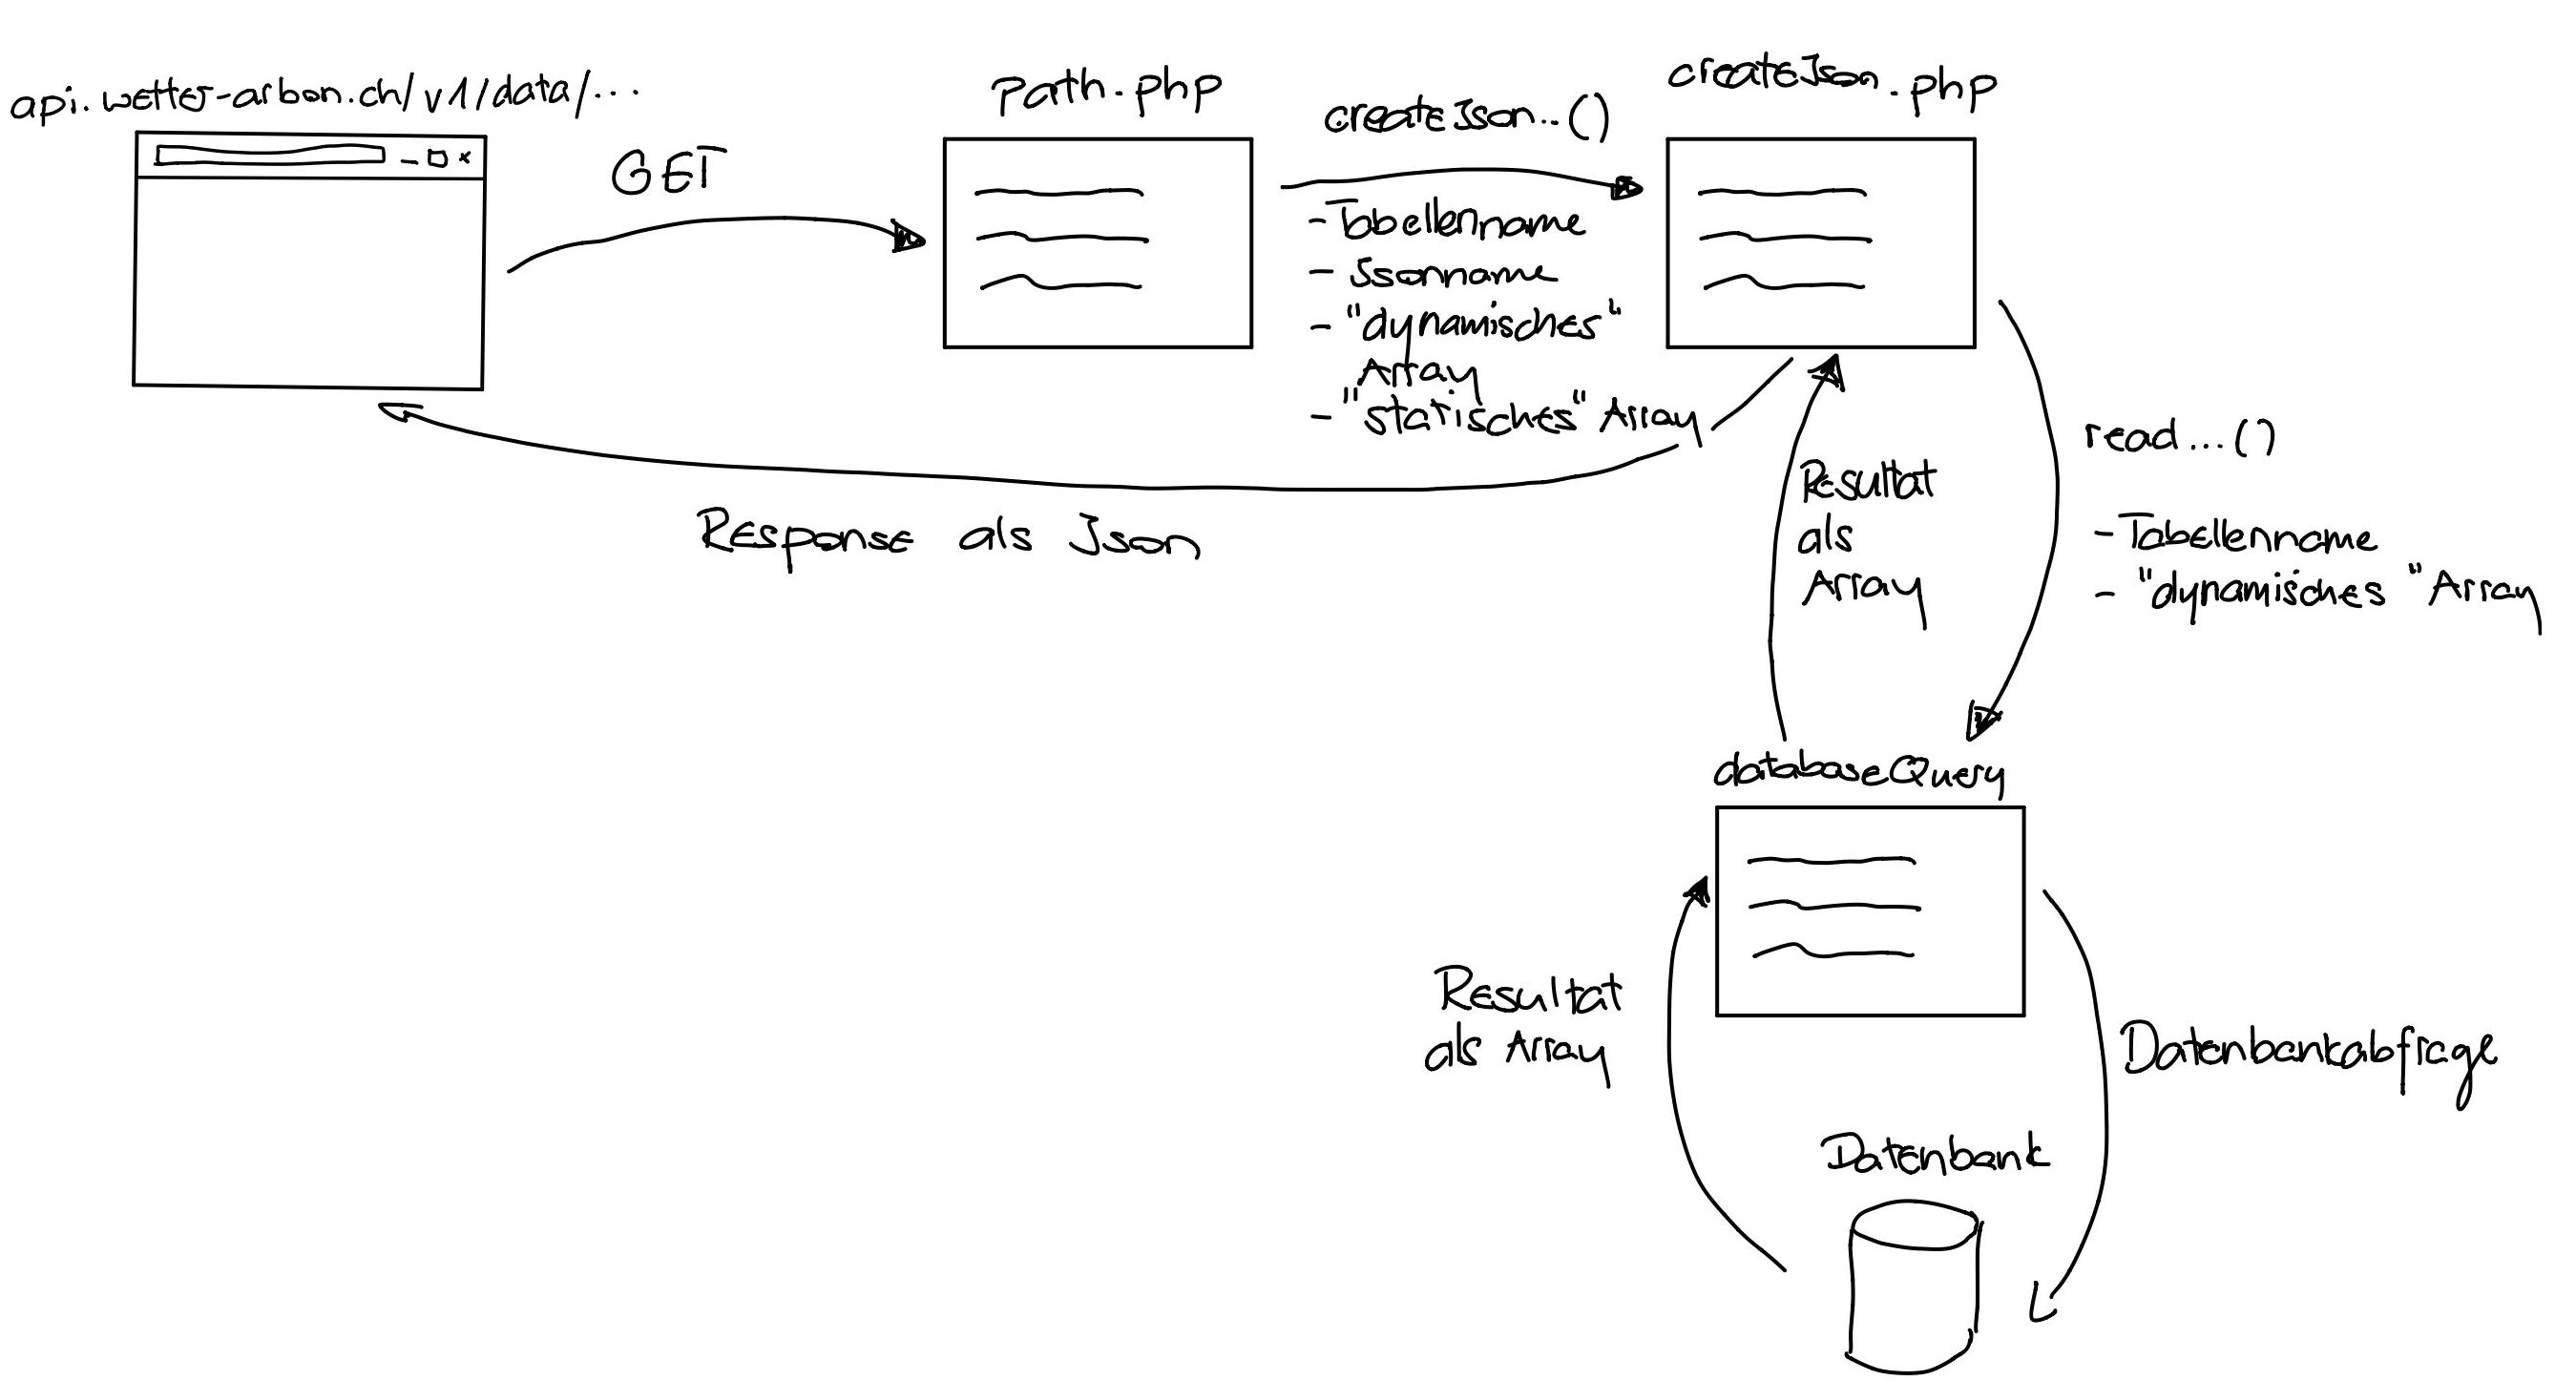
\includegraphics[width=\textwidth-2\fboxsep-2\fboxrule]{img/API_GET.jpg}}
	\centering
	\caption{Ablauf einer API GET-Abfrage}
	\label{img:APIFiles}
\end{figure}

Für die API ist die Datei path.php essentiell (listing \ref{lst:path}). Hier wird wie erwähnt das Routing vorgenommen und die entsprechenden Funktionsaufrufe mit den dazugehörenden Parameter.  


\begin{lstlisting}[label=lst:path,caption=Beispiel Case zuweisung, language=php, style=php]
	...    
    /*Der Case wird nur einmal erklaert da die restlichen vom Aufbau gleich sind*/
        //Ist die URI die gleiche wie fuer den Case wird der Code ausgefuehrt
        case "/v1/misc/east"; //bodensee-east
        //Tabellenname worin die Daten geschrieben sind
        $table = "tblmisc";
        /*Array fuer die Datenbankabfrage wird erstellt.
         Das Array beinhaltet die benoetigten Angaben fuer die Zusammensetzung*/
         $requiredData=array(
          "value" => "warnlevel_east",
          "onset"  => "onset_east",
          "expires" => "NULL"
        );
        /*Das Array mit den statischen Daten wird erstellt.
        Dies wird anschliessend beim zusammensetzen des JSON benoetigt */
        $dataJsonStatic=array(
          "description"  => "Warnlevel east"
        );
        //JSON Name wird vergeben
        $name = "east";
        /*Die entsprechende Funktion um das JSON zu erstellen wird aufgerufen.
        Die vorhin erstellten Arrays sowie variablen werden uebergeben*/
        createJson($requiredData, $dataJsonStatic, $table, $name);
        break;
        ...
\end{lstlisting}

Eine weitere essentielle Datei ist das createJson.php. Hier wird das ganze Json aufgebaut. Für die verschiedenen Arten von Messwerten und deren Ansprüche, sind vier verschiedene Funktionen enstanden:

\begin{itemize}
\item CreateJsonMinMax
\begin{itemize}
\item Diese Funktion erstellt die Jsons mit dem aktuellen Wert sowie den Extrema des Tages
\end{itemize}
\item CreateJson
\begin{itemize}
\item Erstellt das Json für die Daten, welche keine Extrema oder sonstige Umrechnungen benötigen
\end{itemize}
\item CreateJsonConversion
\begin{itemize}
\item Erstellt das Json für die Windgeschwindigkeiten mit den verschiedenen Einheiten Km/h, Knoten und Beaufort. Umgerechnet werden die aktuellen Werte, sowie die Extrema
\end{itemize}
\item createJsonSunduration
\begin{itemize}
\item Rechnet die Sonnenminuten des Tages in Stunden um und erstellt das entsprechende Json Format
\end{itemize}
\end{itemize}

Die Funktionen sind vom Aufbau her alle gleich. Der Unterschied besteht jedoch beim Aufbau des Json. Für einige Messwerte sind Maximal und Minimalwerte gewünscht. Andere Messwerte hingegen werden in verschiedene Einheiten umgerechnet, damit alle Benutzer die Messwerte auch intepretieren können.